% Created 2023-01-25 mié 18:05
% Intended LaTeX compiler: pdflatex
\documentclass[aspectratio=169, usenames,svgnames,dvipsnames]{beamer}
\usepackage[utf8]{inputenc}
\usepackage[T1]{fontenc}
\usepackage{graphicx}
\usepackage{longtable}
\usepackage{wrapfig}
\usepackage{rotating}
\usepackage[normalem]{ulem}
\usepackage{amsmath}
\usepackage{amssymb}
\usepackage{capt-of}
\usepackage{hyperref}
\usepackage{color}
\usepackage{listings}
\usepackage{mathpazo}
\usepackage{gensymb}
\usepackage{amsmath}
\usepackage{diffcoeff}
\usepackage{steinmetz}
\usepackage{mathtools}
\bibliographystyle{plain}
\usepackage{siunitx}
\sisetup{output-decimal-marker={,}}
\DeclareSIUnit{\watthour}{Wh}
\hypersetup{colorlinks=true, linkcolor=Blue, urlcolor=Blue}
\renewcommand{\thefootnote}{\fnsymbol{footnote}}
\newcommand{\laplace}[1]{\mathbf{#1}(\mathbf{s})}
\newcommand{\slp}{\mathbf{s}}
\newcommand{\fasor}[1]{\mathbf{#1}(\omega)}
\newcommand{\atan}{\mathrm{atan}}
\parskip=5pt
\usetheme{Boadilla}
\usecolortheme{rose}
\usefonttheme{serif}
\author{Oscar Perpiñán Lamigueiro}
\date{}
\title{Técnicas Generales de Análisis}
\subtitle{Teoría de Circuitos II}
\setbeamercolor{alerted text}{fg=blue!50!black} \setbeamerfont{alerted text}{series=\bfseries}
\AtBeginSubsection[]{\begin{frame}[plain]\tableofcontents[currentsubsection,sectionstyle=show/shaded,subsectionstyle=show/shaded/hide]\end{frame}}
\AtBeginSection[]{\begin{frame}[plain]\tableofcontents[currentsection,hideallsubsections]\end{frame}}
\beamertemplatenavigationsymbolsempty
\setbeamertemplate{footline}[frame number]
\setbeamertemplate{itemize items}[triangle]
\setbeamertemplate{enumerate items}[circle]
\setbeamertemplate{section in toc}[circle]
\setbeamertemplate{subsection in toc}[circle]
\hypersetup{
 pdfauthor={Oscar Perpiñán Lamigueiro},
 pdftitle={Técnicas Generales de Análisis},
 pdfkeywords={},
 pdfsubject={},
 pdfcreator={Emacs 28.2 (Org mode 9.6)}, 
 pdflang={Spanish}}
\begin{document}

\maketitle

\section{Leyes de Kirchhoff}
\label{sec:org30909ca}

\begin{frame}[label={sec:orgc6c872b}]{Nudo, rama, malla}
\begin{description}
\item[{Nudo}] unión de \alert{3} o más conductores.
\item[{Rama}] elementos conectados entre dos nudos consecutivos.
\item[{Lazo}] conjunto de ramas que forman un camino cerrado.
\item[{Malla}] lazo que no contiene ningún otro en su interior.
\end{description}

\begin{center}
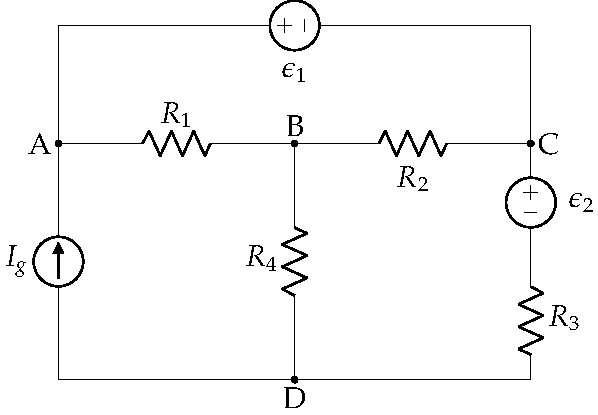
\includegraphics[height=0.5\textheight]{../figs/mallas.pdf}
\end{center}
\end{frame}

\begin{frame}[label={sec:org34d81a7}]{Ley de Kirchhoff de las Corrientes (LKC)}
\begin{itemize}
\item La \alert{LKC} es el principio de conservación de la carga aplicado a los circuitos eléctricos.

\item \alert{LKC}: la suma de las corrientes que llegan a un nudo es igual a la suma de las que salen.

\begin{itemize}
\item Las lineas de corriente son cerradas (o solenoidales).
\end{itemize}
\end{itemize}

\begin{center}
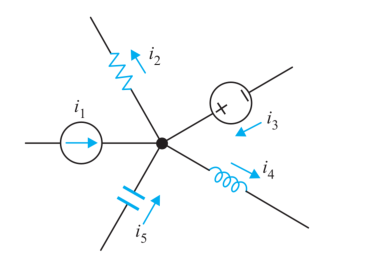
\includegraphics[height=0.4\textheight]{../figs/LKC_FM.pdf}
\end{center}
\[
i_1(t) - i_2(t) + i_3(t) - i_4(t) + i_5(t) = 0
\]
\end{frame}

\begin{frame}[label={sec:orgb37fbfb}]{Ley de Kirchhoff de los Voltajes (LKV)}
\begin{itemize}
\item La \alert{LKV} es el principio de conservación de la energía aplicado a los circuitos eléctricos.

\item \alert{LKV}: la suma (con signo) de las tensiones a lo largo de un camino cerrado (circuito) es cero.

\begin{itemize}
\item La energía producida por un generador es consumida por los receptores del circuito para producir trabajo (mecánico, químico, etc.) o calor.
\end{itemize}
\end{itemize}

\begin{center}
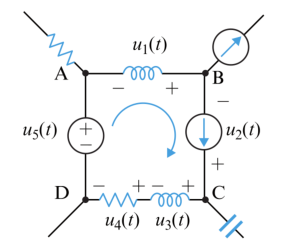
\includegraphics[height=0.4\textheight]{../figs/LKV_FM.pdf}
\end{center}
\[
u_3(t) + u_4 (t) - u_5 (t) - u_1 (t) - u_2 (t)  = 0
\]
\end{frame}

\section{Métodos de Análisis}
\label{sec:orgdbcc74f}

\subsection{Método de las mallas}
\label{sec:org77b94c7}

\begin{frame}[label={sec:org0b86f33}]{}
\begin{center}
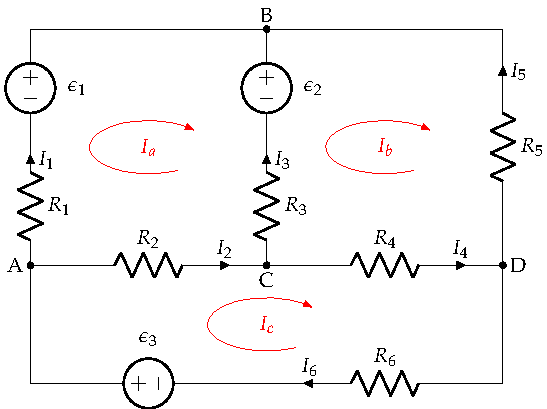
\includegraphics[height=0.95\textheight]{../figs/mallas1_corrientes.pdf}
\end{center}
\end{frame}

\begin{frame}[label={sec:org92beeb3}]{Ecuación General}
\begin{equation*}
  \begin{bmatrix}
    {\color{BrickRed}\sum \overline{Z}_{aa}} &  - {\color{MidnightBlue}\sum \overline{Z}_{ab}} & - {\color{MidnightBlue}\sum \overline{Z}_{ca}} \\
    - {\color{MidnightBlue}\sum \overline{Z}_{ab}} & {\color{BrickRed}\sum \overline{Z}_{bb}} & - {\color{MidnightBlue}\sum \overline{Z}_{bc}} \\
    - {\color{MidnightBlue}\sum \overline{Z}_{ca}} & - {\color{MidnightBlue}\sum \overline{Z}_{bc}} &  {\color{BrickRed}\sum \overline{Z}_{cc}}
  \end{bmatrix} \cdot %
  \begin{bmatrix}
    \overline{I}_a\\
    \overline{I}_b\\
    \overline{I}_c\\
  \end{bmatrix} = %
  \begin{bmatrix}
    {\color{OliveGreen}\sum\overline{\epsilon}_a}\\
    {\color{OliveGreen}\sum\overline{\epsilon}_b}\\
    {\color{OliveGreen}\sum\overline{\epsilon}_c}
  \end{bmatrix}
\end{equation*}
\begin{description}
\item[{\({\color{BrickRed}\sum \overline{Z}_{aa}}\)}] suma de las impedancias incluidas en la malla de \(\overline{I}_a\).
\item[{\({\color{MidnightBlue}\sum \overline{Z}_{ab}}\)}] suma de las impedancias incluidas en las ramas compartidas por las mallas de \(\overline{I}_a\) e \(\overline{I}_b\).
\item[{\({\color{OliveGreen}\sum \overline{\epsilon}_a}\)}] suma algebraica de las fuerzas electromotrices de los generadores de la malla de \(\overline{I}_a\). Su signo es positivo si contribuyen al giro de la corriente.
\end{description}
\end{frame}
\begin{frame}[label={sec:org87f23f9}]{Procedimiento}
\begin{enumerate}
\item Identificar las corrientes de rama.
\item Asignar un sentido a las corrientes de malla.
\item Relacionar corrientes de rama con corrientes de malla.
\item Escribir ecuación de mallas.
\item Resolver la ecuación, obteniendo las corrientes de malla.
\item Obtener las corrientes de rama con las relaciones del punto 3.
\end{enumerate}

\alert{Importante}: todos los generadores deben ser fuentes de tensión.
\end{frame}

\begin{frame}[label={sec:orge96bedd}]{Admitancia generalizada}
\begin{equation*}
  \begin{bmatrix}
    \overline{Z}_{11} & \overline{Z}_{12} & \dots & \overline{Z}_{1n} \\
    \overline{Z}_{21} & \overline{Z}_{22} & \dots & \overline{Z}_{2n} \\
    \vdots & \vdots & \ddots & \vdots \\
    \overline{Z}_{n1} & \overline{Z}_{n2} &  \dots & \overline{Z}_{nn}
  \end{bmatrix} \cdot %
  \begin{bmatrix}
    \overline{I}_1\\
    \overline{I}_2\\
    \vdots \\
    \overline{I}_n\\
  \end{bmatrix} = %
  \begin{bmatrix}
    \overline{\epsilon}_1\\
    \overline{\epsilon}_2\\
    \vdots \\
    \overline{\epsilon}_n
  \end{bmatrix}
\end{equation*}
Aplicando la regla de Cramer
\[
  \overline{I}_k = \overline{\epsilon}_1 \frac{\Delta_{1k}}{|Z|} + \overline{\epsilon}_2 \frac{\Delta_{2k}}{|Z|} + \dots + \overline{\epsilon}_n \frac{\Delta_{nk}}{|Z|}
\]
siendo \(\Delta_{ij}\) el adjunto del elemento \(ij\) de la matriz \(Z\):
\[
  \Delta_{ij} = (-1)^{i+j} \cdot |M_{ij}|
\]
donde \(M_{ij}\) es la matriz resultante de eliminar la fila \(i\) y la columna \(k\) de la matriz \(Z\).
\end{frame}

\begin{frame}[label={sec:orgc7c5c8d}]{Admitancia generalizada}
Esta expresión indica que las respuestas del circuito (\(I_k\)) dependen de todas las excitaciones que existan (\(\epsilon_i\)):
\[
  \overline{I}_k = \overline{\epsilon}_1 \frac{\Delta_{1k}}{|Z|} + \overline{\epsilon}_2 \frac{\Delta_{2k}}{|Z|} + \dots + \overline{\epsilon}_n \frac{\Delta_{nk}}{|Z|}
\]
También se puede definir la admitancia generalizada entre dos partes del circuito:
\[
  \overline{Y}_{ki} = \frac{\overline{I}_k}{\overline{\epsilon}_i} = \frac{\Delta_{ik}}{|Z|}
\]
\end{frame}

\begin{frame}[label={sec:orgcfd2570}]{Impedancia de Entrada}
A partir de esta expresión se puede calcular la impedancia de entrada vista por una fuente que alimenta un circuito pasivo (todas las fuentes salvo la de entrada son nulas en la expresión anterior):

\[
  \overline{I}_1 = \overline{\epsilon}_1 \frac{\Delta_{11}}{|Z|} + 0 \cdot \frac{\Delta_{21}}{|Z|} + \dots + 0 \cdot \frac{\Delta_{n1}}{|Z|}
\]
Por tanto:
\[
  \boxed{\overline{Z}_{in} = \frac{\overline{\epsilon}_1}{\overline{I}_1}=  \frac{|Z|}{\Delta_{11}}}
\]
\end{frame}

\begin{frame}[label={sec:org7e38cd2}]{Impedancia de Transferencia}
También se puede calcular la impedancia de transferencia de un circuito pasivo, es decir, la impedancia entre dos partes del circuito en las que la primera está alimentada por una fuente, y la segunda está cortocircuitada.

En este caso, todas las fuentes salvo la de interés están apagadas:

\[
  \overline{I}_k = 0 \cdot \frac{\Delta_{1k}}{|Z|} + 0 \cdot \frac{\Delta_{2k}}{|Z|} + \dots + \epsilon_j \cdot \frac{\Delta_{jk}}{|Z|} + 0 \cdot \frac{\Delta_{nk}}{|Z|}
\]
Por tanto:
\[
  \boxed{\overline{Z}_{Tjk} = \frac{\overline{\epsilon}_j}{\overline{I}_k}=  \frac{|Z|}{\Delta_{jk}}}
\]
\end{frame}


\begin{frame}[label={sec:orga1f3869}]{Mallas con fuentes de intensidad}
\end{frame}
\begin{frame}[label={sec:org590956b}]{Mallas con fuentes dependientes}
\end{frame}

\subsection{Método de los nudos}
\label{sec:orgac60dda}
\begin{frame}[label={sec:orgb4d0e4c}]{}
\begin{center}
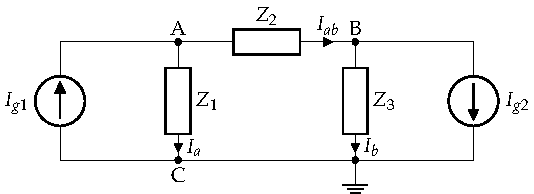
\includegraphics[width=.9\linewidth]{../figs/nudosAC.pdf}
\end{center}
\end{frame}

\begin{frame}[label={sec:org3e67492}]{Ecuación general}
\begin{equation*}
  \begin{bmatrix}
    {\color{BrickRed}\sum \overline{Y}_A} & - {\color{MidnightBlue}\sum \overline{Y}_{AB}} & - {\color{MidnightBlue}\sum \overline{Y}_{AC}}\\
    -{\color{MidnightBlue}\sum \overline{Y}_{AB}} & {\color{BrickRed}\sum \overline{Y}_B} & -{\color{MidnightBlue}\sum \overline{Y}_{BC}}\\
    -{\color{MidnightBlue}\sum \overline{Y}_{AC}} & -{\color{MidnightBlue}\sum \overline{Y}_{BC}} & {\color{BrickRed}\sum \overline{Y}_C}
  \end{bmatrix} \cdot%
  \begin{bmatrix}
    \overline{V}_A\\
    \overline{V}_B\\
    \overline{V}_C
  \end{bmatrix} = %
  \begin{bmatrix}
    {\color{OliveGreen}\sum \overline{I}_{gA}}\\
    {\color{OliveGreen}\sum \overline{I}_{gB}}\\
    {\color{OliveGreen}\sum \overline{I}_{gC}}
  \end{bmatrix}
\end{equation*}

\begin{description}
\item[{\({\color{BrickRed}\sum \overline{Y}_A}\)}] Suma de las admitancias conectadas al nudo \(A\).
\item[{\({\color{MidnightBlue}\sum \overline{Y}_{AB}}\)}] Suma de las admitancias conectadas entre los nudos \(A\) y \(B\).
\item[{\({\color{OliveGreen}\sum \overline{I}_{gA}}\)}] Suma de las corrientes de los generadores conectados en el nudo A. El signo es positivo si el generador inyecta corriente en el nudo.
\end{description}

\alert{Importante}: todos los generadores deben ser fuentes de corriente.
\end{frame}


\begin{frame}[label={sec:org1ad7455}]{Impedancia Generalizada}
Diapositiva 18 de JP
\end{frame}

\begin{frame}[label={sec:orgf9dbd30}]{Admitancia de Entrada}
\end{frame}

\begin{frame}[label={sec:org63bb4df}]{Admitancia de Transferencia}
\end{frame}

\begin{frame}[label={sec:org1dbf72e}]{Supernudos}
\end{frame}
\end{document}